\begin{frame}{How to use WebRTC}
\begin{tikzpicture}
\node at (0,0) {\includegraphics[page=9,height=\textheight]{image/webrtc.pdf}};
\node[align=center, nounibaredII] at (4.5,1) {A few lines of\\ JavaScript is all\\ that is needed!};
\end{tikzpicture}
\end{frame}

\begin{frame}{WebRTC Peer-to-Peer Media}\framesubtitle{Media Flows in WebRTC}
\begin{figure}
\includegraphics[page=10,width=\textwidth]{image/webrtc.pdf}
\end{figure}
\end{frame}

\begin{frame}{WebRTC Peer-to-Peer Media}\framesubtitle{Media without WebRTC}
\begin{tikzpicture}
\node at (0,0) {\includegraphics[page=11,width=\textwidth]{image/webrtc.pdf}};
\node[align=center, nounibaredII] at (-3,-3) {A browser plug-in must be used};
\end{tikzpicture}
\end{frame}

\begin{frame}{WebRTC Peer-to-Peer Media}\framesubtitle{Peer-to-Peer Media with WebRTC}
\begin{tikzpicture}
\node at (0,0) {\includegraphics[page=12,width=\textwidth]{image/webrtc.pdf}};
\node[align=center, nounibaredII] at (-3,-3) {No plug-in or download required!};
\end{tikzpicture}
\end{frame}

\begin{frame}{WebRTC Peer-to-Peer Media}\framesubtitle{NAT Complicates Peer-to-Peer Media}
\begin{tikzpicture}
\node at (0,0) {\includegraphics[page=13,width=\textwidth]{image/webrtc.pdf}};
\node[align=center, nounibaredII, font=\footnotesize] at (3.5,-3.5) {Most browsers are behind NATs\\ on the Internet, which\\ complicates the establishment\\ of peer-to-peer media sessions};
\node[align=center, nounibaredII] at (-3,-3) {Network Address Translator};
\end{tikzpicture}
\end{frame}

\begin{frame}{WebRTC Peer-to-Peer Media}\framesubtitle{NAT Media Through NAT}
\begin{tikzpicture}
\node at (0,0) {\includegraphics[page=14,width=\textwidth]{image/webrtc.pdf}};
\node[align=center, nounibaredII, font=\footnotesize] at (3.5,-3.5) {ICE hole punching can often\\ establish a direct peer-to-peer\\ session between browsers\\ behind different NATs};
\node[align=center, nounibaredII] at (-3,-3) {Interactive Communications\\ Establishment, RFC 5245};
\end{tikzpicture}
\end{frame}

\begin{frame}{High Level ICE Call Flow}
\begin{columns}
\column{.7\textwidth}
\begin{figure}
    \resizebox{1\textheight}{!}{
    	\begin{scriptsize}
\begin{sequencediagram}
  \newthread[0]{unibagrayI}{a}{Agent A}
  \newthread[0]{white}{n1}{NAT}
  \newthread[3]{unibablueV}{s}{STUN Server} 
  \newthread[3]{white}{n2}{NAT} 
  \newthread[0]{unibagrayIII}{b}{Agent B}
  
  \mess[0]{a}{1 Gather transport addresses}{s}
  \mess[0]{a}{2 Offer}{b}
  \mess[0]{b}{1 Gather transport addresses}{s}
  \mess[0]{b}{2 Answer}{a}
  \mess[0]{a}{3 STUN check}{b}
  \mess[0]{b}{3 STUN check}{a}
  \mess[0]{a}{4 Media}{b}
  \mess[0]{b}{4 Media}{a}
  \mess[0]{a}{5 Keep-Alive}{b}
  \mess[0]{b}{5 Keep-Alive}{a}
 
\end{sequencediagram}
\end{scriptsize}
    }
    \begin{tiny}
       Transport address is IP address and port number
     \end{tiny}
\end{figure}
\column{.3\textwidth}
\begin{tiny}
\begin{enumerate}
\item Gather candidate transport addresses
\item Exchange candidates over signaling channel
\item Perform connectivity checks
\item Choose selected pair and begin media transport
\item Send keep-alives
\end{enumerate}
If either side detects a change iin IP address in use, ICE is restarted (back to step 1)
\end{tiny}
\end{columns}
\end{frame}

\begin{frame}{WebRTC Peer-to-Peer Media}\framesubtitle{P2P Media Can Stay Local to NAT}
\begin{tikzpicture}
\node at (0,0) {\includegraphics[page=15,width=\textwidth]{image/webrtc.pdf}};
\node[align=center, nounibaredII, font=\footnotesize] at (3.5,-3.5) {If both browsers are behind the\\ same NAT, hole punching can\\ often establish a connection\\ that never leaves the NAT};
\end{tikzpicture}
\end{frame}

\begin{frame}{WebRTC Peer-to-Peer Media}\framesubtitle{Browser Queries STUN Server}
\begin{tikzpicture}
\node at (0,0) {\includegraphics[page=16,width=\textwidth]{image/webrtc.pdf}};
\node[align=center, nounibaredII, font=\footnotesize] at (3.5,-3.5) {Browser sends STUN test\\ packet to STUN server to\\ learn its public IP address\\ (address of the NAT)};
\node[align=center, nounibaredII] at (-3,-3) {Session Traversal Utilities\\ for NAT, RFC 5389};
\end{tikzpicture}
\end{frame}

\begin{frame}{WebRTC Peer-to-Peer Media}\framesubtitle{TURN Server Can Relay Media}
\begin{tikzpicture}
\node at (0,0) {\includegraphics[page=17,width=\textwidth]{image/webrtc.pdf}};
\node[align=center, nounibaredII, font=\footnotesize] at (3.5,-3.5) {In some cases, hole punching\\ fails, and a TURN Media Relay\\ on the public Internet must be used.};
\node[align=center, nounibaredII] at (-3,-3) {Traversal of UDP\\ aRound NAT, RFC 5766};
\end{tikzpicture}
\end{frame}